\documentclass[12pt,a4paper]{article}
\usepackage{color, colortbl}
\definecolor{Gray}{gray}{0.8}
\definecolor{LightRed}{rgb}{0.99,0.9,0.9}
\usepackage{graphicx}
\usepackage{algpseudocode}
\usepackage{graphicx}
\usepackage{url}
\usepackage{verbatim}
%\usepackage{caption}
%\usepackage{subcaption}
%\usepackage{textcomp}
%\usepackage{fancyvrb}
\usepackage{graphicx}
\usepackage{amssymb}
\usepackage{epstopdf}
\usepackage[nottoc,numbib]{tocbibind}
\usepackage[
      pass
]{geometry}

\newcommand\todo[1]{\textcolor{red}{#1}}

\begin{document}
\title{\small Project Proposal\\\huge Investigating Methods Of Annotating Lifelogs For Use In Search}

\author{Harry Scells - 8857580\\harrisen.scells@connect.qut.edu.au\\\\\small Supervisor - Guido Zuccon\\\small g.zuccon@qut.edu.au\\}
\maketitle
\pagebreak
\tableofcontents
\pagebreak

\section{Introduction}
Digitally recording and documenting life and daily activities is becoming increasingly popular. One such activity which enables this is lifelogging, which encapsulates a wide range of devices and sensors. Gurrin et al.~\cite{gurrin2014lifelogging} argue that lifelogging is an emergent area of research which is filled with terminology that is not well considered and defined, and as such, defines lifelogging as "the process of passively gathering, processing, and reflecting on life experience data collected by a variety of sensors, and is carried out by an individual, the lifelogger. The life experience data is mostly based on wearable sensors which directly sense activities of the person, though sometimes data from environmental sensors or other informational sensors can be incorporated into the process". Primarily, lifelogging involves an image capture device attached to a shirt or a lanyard which takes several photos a minute.

The problem that arises here is searching through the vast number of images taken each day. This is the basis for the NTCIR Lifelogging pilot task, and consequently this research. The focus for this research project is to investigate different annotating methodologies for use in searching lifelog images. Well formed, accurate annotations are a critical aspect to a collection of lifelog images. This is why the project focuses not on searching images, but developing an annotated collection. This will be an important contribution to the community of lifelog information retrieval as the current annotations for lifelog images are of poor quality.

\section{Preliminary Literature Review}
% ---------------------------------
%  BEGIN LIT REVIEW
% ---------------------------------
\subsection{Representing the Data Through Modelling Human Memory}
One way of viewing lifelogging is the process of creating a surrogate memory for a person. Organising and presenting are the key challenges for lifelog search engines. Gurrin et al.~\cite{gurrin2014lifelogging} proposes that it is possible to segment the raw, unprocessed lifelog data into meaningful units, or events; which he defines as: "a temporally related sequence of lifelog data over a period of time with a defined beginning and end". In order to perform information retrieval, the events need to be annotated with meaningful semantics. Annotations can either be manually created by humans, or generated through machine learning algorithms. These annotations must also be evaluated for effectiveness, as poor annotations will lead to poor performance when performing retrieval on the images.

There are five aspects of human memory access, as proposed by Gurrin et al.~\cite{gurrin2014lifelogging}:
\begin{enumerate}
    \item Recollecting: Concerned with re-living and accessing past experiences of episodic memories.
    \item Reminiscing: A form of recollecting, concerned with reliving past experiences for emotional or sentimental reasons.
    \item Retrieving: A more specific form of recollecting  in which specific information needs are to be retrieved such as an address, a document, a location, or any atomic piece of information.
    \item Reflecting: A form of quantified-self analysis, performed in order to discover knowledge and insights that may not be immediately obvious.
    \item Remembering: Concerned with prospective memory more than episodic memory. A form of planning for future activities or to act as a reminder or prompt for tasks that a person would like to do.
\end{enumerate}
Gurrin et al.~\cite{gurrin2014lifelogging} argues that an information retrieval system targeted at lifelogging should focus on the Five R's as information needs for the user.

In the context of searching images on the web,  L. Vuurpij, et al.~\cite{vuurpij2002vind} states that image retrieval systems are restricted to the domain they cover and require a lot of domain knowledge in order to fulfill the information needs of a user. Furthermore, L. Vuurpij, et al.~\cite{vuurpij2002vind} notes that there has been a shift from computer vision and pattern recognition to psychology and cognitive science in the domain of image retrieval, where models like the Five R's~\cite{gurrin2014lifelogging}, are becoming more prevalent. 

\subsection{Annotating Lifelog Images}
The current state of the art models for image retrieval use tag-based or textual description annotations \citep{ali2010semantically}. This is typically due to the fact that retrieval models can use this text as a bag of words, or use the text to attribute some form of semantic meaning.

\subsubsection{Evaluating Annotations}
Without high quality annotations, semantic search would not work, since semantic search exploits the meaning and context of a sentence rather than the keywords in it \cite{ali2010semantically}. The semantic and contextual data associated with images is important for an effective retrieval model that uses textual features rather than pixel data in images. This textual data can either be generated using machine learning algorithms, as demonstrated by A. Karpathy et al.~\cite{karpathy2015deep} and  I. Sutskeve et al.~\cite{sutskever2011generating}, or generated manually by humans. The machine learning algorithms do however start from test data, typically of a specific domain or a range of domains, which they learn from. It is important to note that this can have undesirable consequences when trying to apply a model which has been trained on one domain to one which it has no knowledge of. In both situations, it is essential that the annotations themselves are evaluated such that they describe the image with enough detail and are convincing to humans, since queries will be formulated by humans. Three widely used models for this exist: BLEU \citep{papineni2002bleu} which is precision based, ROUGE (Recall-Oriented Understudy for Gisting Evaluation) \citep{lin2004rouge} which is recall based, and METEOR \citep{elliott2013image}, used for judging the overall quality of annotations.

All of the metrics above were initially proposed with respect to the evaluation of automatic summarisation and natural language processing. Furthermore, they all use a reference annotation in order to score annotations. ROUGE compares the number of overlapping n-grams, word sequences, and word pairs of annotations with ideal annotations created by humans \citep{lin2004rouge}. BLEU counts the maximum number of times a word appears in any reference annotation, followed by "clipping" the total count of each candidate word by its maximum reference count, adding these "clips" up, and dividing by the total unclipped number of candidate words in the annotation \citep{papineni2002bleu}. The notion of "clipping" in BLEU is a variation of precision whereby words are only accepted for the maximum number of times they appear the reference text, for instance if a word appears in an annotation five times but is in the reference annotation twice, the "clipped" value would be 2/5. Finally, METEOR generally operates by unigram matching (bag of words) between a reference annotation, typically created by a machine, and a human produced annotation. Both METEOR and ROUGE take multiple approaches to comparing annotations, for reference, ROUGE:
\begin{enumerate}
    \item ROUGE-N N-gram Co-occurence Statistics
    \item ROUGE-L Longest Common Subsequence
    \item ROUGE-W Weighted Longest Common Subsequence
    \item ROUGE-S Skip-Bigram Co-Occurence Statistics
    \item ROUGE-SU Skip-Bigram Co-Occurence Statistics with Unigram Counting Unit
\end{enumerate}
The unigrams matched in METEOR can be based on surface forms, stemmed forms, and meanings, with the option to be extended \citep{elliott2013image}.

R. Vedantam et al.~\citep{vedantam2015cider} argue through the results of their experimentation, however, that there exists a more effective model for evaluation which is rooted in human consensus. Their method, CIDEr (Concensus-based Image Description Evalutation) is a model which outperforms all other models of evaluating descriptive annotations of images. CIDEr performs so well due to high correlation with human judgement and consensus. According to R. Vedantam et al.~\cite{vedantam2015cider}, the CIDEr metric inherently captures sentence similarity, the notions of grammatically, salience, importance (precision), and accuracy (recall). CIDEr appears to improve upon the other three models and takes into account the weaknesses the other models may have, however it still relies on reference annotations.

The evaluation methods above rely on the availability of a ground truth or reference annotation that can be used to compare with the automatically generated annotation. This approach, however, is ill-suited to generating annotations for lifelog images as it is unclear what these annotations should ``look like'', because it is unknown what makes an annotation of a lifelog image ``good''. A better suited alternative for this problem is to embed the evaluation of different annotation methods within a task and thus evaluate the  methods with respect to the effectiveness the different methods induce on the task. Specifically, in this research project, the aim is to embed the evaluation of lifelog annotation within a search task. Thus the effectiveness of a system would be evaluated with respect to the search task. None of the system properties would vary apart from the method that is used to annotate images.This evaluation methodology is akin to, for example, previous work that has examined the effectiveness and quality of different topic modelling techniques and semantic models via evaluating the effect they have on search engine result effectiveness~\cite{wei2006lda,zuccon2015integrating,karimzadehgan2010estimation,yi2009comparative}.

\subsubsection{Types of Annotations}
As suggested by R. Yan et al.~\cite{yan2008learning}, the most common image annotation approaches can be categorised into two types. The first is \textit{tagging}, where annotators choose a set of keywords from a vocabulary for each image. The second most common approach is described as \textit{browsing}, where a group of images are judged against the relevance of a predefined keyword. There are, however, less commonly used annotation approaches, for example, \textit{descriptive natural language annotations} which are generated in a model by A. Karpathy et al.~\cite{karpathy2015deep}. This model outperforms the previous work done in this area of research for both image retrieval and image annotation on the Flickr8K, Flickr300K and MSCOCO. B. Hu et al.~\cite{hu2003ontology} clarifies why high quality textual descriptions generally perform better than systems that employ keyword or tag based annotation models, in that these models suffer from several limitations:
\begin{enumerate}
    \item A keyword in a document does not necessarily mean that the document is relevant
    \item A relevant document may not contain the explicit word
    \item Synonyms of the query keywords lower the recall rate (ratio of retrieved images which are relevant to the total number of relevant images, see Appendix A for details)
    \item Homonyms of the query keywords lower the precision rate  (ratio of relevant images that are successfully retrieved to the total number of relevant and irrelevant images retrieved) see Appendix A for details)
    \item Semantic relations such as hyponymy, meronymy, antonymy are not exploited
\end{enumerate}

Recent work in the consumer health search domain by Zuccon et al.~\cite{quteprints82599} and Stanton et al.~\cite{stanton2014circumlocution} focused on generating queries from images. The aim of their research was to understand how the general public would search for information if they had a medical condition as that in the image presented to them. This new methodology used by these previous works could be adapted to the context of gathering annotations for lifelogging, thus leading to an \textit{annotation by querying} method. This method would consist of showing annotators an image from a lifelogger and ask them to provide the queries they would issue to a (standard) search engine to attempt to retrieve the image itself.

\subsection{Searching for Lifelog Images}
Lifelog information retrieval systems typically have very poor performance due to there not being any formal models made specifically for the field, as reported by Gurrin et al.~\citep{gurrin2014lifelogging}. Until very recently, there have been no large, distributable test collections such as the TREC collection for text \citep{gurrin2014lifelogging}. The NTCIR collection is a set of tagged lifelog images which have been collected by researchers who wore a lifelogging camera for a short amount of time \citep{gurrin2016ntcir}. The tags were automatically generated by using a pre-trained image tagging algorithm.

While there is limited applied methodology to retrieval models in lifelogging, there has been much discussion about what the models should try and solve. Both H.  W.  Bristow et al.~\citep{bristow2004defining} and A. R. Doherty et al.~\cite{doherty2010automatically} corroborate that detecting and interpreting the implicit semantics and context of lifelogging data from heterogeneous sources would be advantageous in explaining the Who?, What?, Where? and When? questions which occur in every day events. It was also noted that these questions are common among image searchers and that they are not capable of being answered by normal indexing like that in traditional search engines \citep{ali2010semantically}.

While there has been some research into tagging and annotating images, there has not been as much work in developing a model for searching these images within the context of lifelogging \citep{gurrin2014lifelogging}. Typical image search engines for web pages treat the surrounding text, captions, alternate text and HTML titles \citep{frankel1996webseer} as a bag of words for retrieval. The success of these search engines rely on a sufficient amount of surrounding text, something which is not provided by current automatic image annotation models for lifelogging. The longer and more detailed the text is within the context of the image, the better the performance of the search engine. This is perhaps why other research has involved novel search techniques \citep{vuurpij2002vind}, since the current models for generating captions of images are not yet detailed or accurate enough for current textual information retrieval models to work.

% ---------------------------------
%  END LIT REVIEW
% ---------------------------------

\section{Research Questions}
The literature reviewed has revealed a gap in the research that nobody else has yet addressed. Annotation of lifelog images and the evaluation of them is not a standard process. Through preliminary research, I have investigated a number of techniques which are applicable to annotating images. A number of textual summarisation evaluation methods have also been discovered, however none of these are capable of evaluation without a ground truth or gold standard. Through researching the following two questions, it is hoped that these gaps in the research can be closed.

\paragraph{RQ1:} How can annotations for a collection of lifelog images be evaluated?
It is important that the annotations of images are accurate and of a high quality. This will need to be done without using a gold standard annotation, since this does not exist. In this way, this research will identify a novel way of evaluating annotations for lifelog images. The most promising way to do this is through extrinsic evaluation, whereby annotations are evaluated by determining the performance of a bigger system using it.

\paragraph{RQ2:} What are the possible ways lifelog images can be annotated?
There are many state of the art solutions for automatically summarising the contents of images, however this project will involve manual annotations. This is due to the fact that there does not exist any training data specifically for lifelog images. This makes it challenging to train a model that can identify what is in a lifelog image. It is thought that by manually annotating images, a well formed collection of annotated lifelog images can be produced, as well as data which machine learning and computer vision algorithms can exploit.

\section{Aims}
When images have annotations, it is possible to apply existing textual information retrieval techniques to search them. Annotating images allows us to represent them in some textual form (as a document). This project consists of two aims: investigating lifelog image annotation methodologies and develop an evaluation metric for each of the types of annotations.

Image annotation approaches exist, however these methodologies do not have any associated literature which analyse the effectiveness of them within the context of a lifelog collection. The methods of annotation under investigation are:
\begin{enumerate}
    \item Image Tagging
    \item Image Browsing
    \item Annotation by Descriptive Text
    \item Annotation by Reverse Query
\end{enumerate}
Each annotation methodology requires an image annotation interface in order to collect annotations. Generating annotations for lifelog images is unreliable even when using state of the art machine learning software. It is for this reason that manual collection of annotations is preferred. The CAFFE concepts list, distributed with the lifelog image collection, demonstrates this unreliability and subsequent poor search performance. Images annotations comprise of concepts of what the software sees, however this is inaccurate. The training data used does not suite the test data, and a consequence of this is many erroneous concepts.

Evaluation of the effectiveness of each methodology will occur after the collection of a substantial number of annotations. The evaluation system will operate in a similar manner to topic modelling where evaluation is embedded in a search task.  The search engine will not change between each evaluation, the only factor that changes is the annotation type. The retrieval effectiveness dictates the efficiency of the annotation methodology. 

\section{Methodology}
\subsection{Evaluation Of Image Annotations}
Typical image summarisation evaluation metrics make use of a reference or gold standard annotation. Since it is unknown what an annotation of a lifelog image should look like, these types of metrics are unable to be used in this project. Hence this is why the project will employ extrinsic evaluation. The evaluation of lifelog images will be embedded in a search task, much like how topic models are evaluated. The effectiveness of an annotation will be evaluated with respect the the search task. In this way, a search engine to facilitate this evaluation will be built.

The search engine that is used in the evaluation of annotations must be able to retrieve images using the four different annotation methods outlined in this proposal. The queries used to test the effectiveness of the annotations will be taken from the NTCIR pilot task. These queries were compiled by asking lifeloggers to recollect what they thought were significant moments from their time capturing data.

Each annotation type will need to be retrieved and ranked independently to each other. Since the retrieval model can influence the evaluation, a set of baseline retrieval models will be tested to weigh out the differences. The proposed evaluation methods are outlined below.

\paragraph{Evaluating Tags}
The search engine will retrieve images using tags by first tokeninsing the query, followed by retrieving images using a binary model, and finally ranking each image by weighing images with respect to the query. If a tag appears on an image, it must be relevant, and if a tag does not appear on an image it must not be relevant. When ranking images, they can be weighted by calculating the number of relevant and non-relevant tags that appear with respect to the query. An image will be more relevant to a query if more of its tags appear in the query. One difficulty with this measure is accounting for the number of tags an image has. If an image has relevant tags but many non-relevant tags, it may rank lower than an image with the same amount or less relevant tags, with less tags overall.

\paragraph{Evaluating Browsing Annotations}
Browsing annotations are retrieved by first tokenising the query, followed by retrieving images that have concepts contained in the query, and finally ranking by weighting each image using the relevance assigned to each concept. Images will be retrieved in much the same way as the tag-based approach. If a concept has a relevancy score of zero, it will be considered the same as if a tag is not present. An image will be more relevant to a query if more of it's concepts are relevant to a query, and if those concepts have a higher relevance to the image.

\paragraph{Evaluating Textual Descriptions}
Textual descriptions are retrieved in a similar manner to typical text based retrieval methods. The textual description is treated as a vector, where each word in the vector is weighted using term frequency-inverse document frequency (tf-idf). The query is also encoded into a vector, so ranking and retrieving images is done in one step. The cosine similarity of the query vector and each description vector is calculated to produce a search listing.

\paragraph{Evaluating Reverse Queries}
A well established method of retrieving documents that are composed of reverse queries does not exist since it is an unexplored research area. Methods for retrieving and ranking reverse queries will be investigated as part of this project. One possible way of retrieving images that contain this type of annotation could be to perform some type of query expansion in conjunction with a retrieval model similar to that used for textual descriptions.

\subsection{Methods of Annotation}
In order for annotations to be collected for each of the annotation methodologies, an interface for each one must be developed. Each interface will allow users to annotate one image at a time at random from a queue of images to be annotated. 

These interfaces will be made available through a web front end, allowing it to be accessible by anyone involved at any time. A database will be used to store the annotations for later evaluation.

\paragraph{Tagging Interface}
The tagging interface will allow annotators to attach tags from a vocabulary. This vocabulary will initially be comprised of tags from the set of queries distributed with NTCIR. Arbitrary tags may be added to the vocabulary at will. Similar tags will also be generated using word2vec. One image at a time will be shown to a user and they will be able to choose tags from a list as thye type.

\begin{center}
    \includegraphics[width=390px]{images/tagging}
\end{center}

Similar tags will be shown underneath the search bar. As tags are added to an image, they will display nearby. This will allow the user annotating to see what they have added so far. By allowing the annotator to see similar tags, it is hoped that they will add more tags. 

The annotations for this method are the tags that a user adds to the image. Once an annotation has finished tagging an image, another new image is shown. Images may only be tagged once.

\paragraph{Browsing Interface}
The image browsing interface will show a number of images and the user will judge the relevance of the images with relation to a keyword.

\begin{center}
    \includegraphics[width=390px]{images/browsing}
\end{center}

The user will be provided with one image at a time, and a relevance scale. The user is asked to judge how relevant a given concept is to the target image. 

Each image will have a set of associated concepts which are weighted on a ten point scale with zero being not relevant, five being relevant, and ten being highly relevant. This interface has a set of buttons ranging from zero to ten from which the user annotating may judge. After an annotator has selected a relevance score, either the same image with a different concept, a new image with a different concept, or a new image with the same concept will appear. No image will have the same concept judged more than once, but some images may have more concepts than others.

\paragraph{Descriptive Text Interface}
The descriptive text interface will present the user with one image at a time. The user is then asked to provide a detailed description for the image.

\begin{center}
    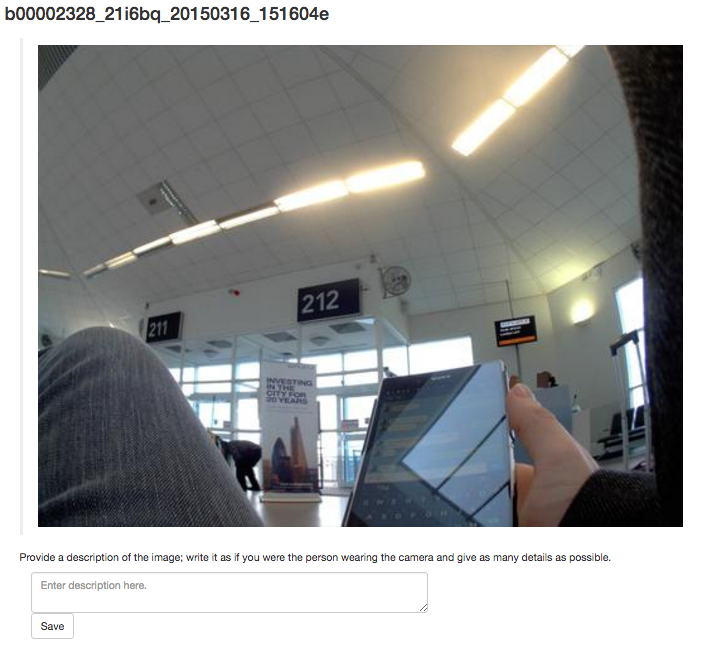
\includegraphics[width=390px]{images/descriptive}
\end{center}

This interface has already been implemented through preliminary research. This annotation method was chosen because it was thought that semantic meaning and concepts can be extracted from long form text. It was found that some users would enter annotations too short to gain any sort of semantics from it, thus some more work must be done to prevent this. Images are only annotated once.

\paragraph{Reverse Query Interface}
The reverse query interface will operate in a manner very similar to the descriptive text interface. Rather than being asked to provide a detailed description for each image, the user will be asked to enter one or more queries that they believe would result in a search engine retrieving the image.

\begin{center}
    \includegraphics[width=390px]{images/reverse-query}
\end{center}

The user is presented with a similar interface to a commercial search engine. The difference here is that the images are already retrieved and the user must enter a query which he or she thinks would cause the images to be retrieved. Images are only annotated once.
 
\subsubsection{Image Sampling}
Sampling images for annotation is necessary due to the large nature of the collection. One naive approach might be to randomly sample images for annotation. This method would not capture enough variation for a small number of annotations. A better approach~\cite{harry2016lifelog} is to use a cluster based sampling technique. Visually and temporally similar groups of images can be clustered and are able to be sampled from this. this method provides a much more even distribution of images to annotate.

\subsubsection{Annotation Requirements}
The collection of images is too large for every image to be annotated at least once for each of the annotation methodologies. Therefore a measure of how many annotations needed must be calculated. Since it is expected that only one person will provide annotations, this will be a major contributing factor to the number of annotations that can be collected.

If more people are required to provide annotations due to time constraints, there are two options for recruiting humans for annotating images: students and staff at QUT or Amazon Mechanical Turk. The Mechanical Turk is an online service offered by Amazing. It allows researchers and companies to issue tasks to people. The people performing the annotations through this method may not have high English comprehension skills, which is a critical factor for high quality annotations. On the other hand, it will be difficult to recruit QUT students and staff to annotate images, since it is a very time consuming process.

\section{Significance}
There are no known studies in the literature which have collected a suitable collection of annotations for lifelog images. The culmination of this research will accelerate the development of lifelog centric search engines by providing a test collection to use as the basis for a search engine and to train predictive models and classifiers. Current state of the art image retrieval algorithms~\cite{karpathy2015deep} rely on training data in order to create unsupervised models that can in turn be used to classify the contents of images. If a training data set is not suited to the test set, it is likely that false positives and misclassifications will occur. Since humans will be collecting annotations, rather than other automated approaches, it is hoped that the annotations for a training set will be higher quality and more accurate than automatic annotation techniques. 

Until recently, there has been a lack of a readily available, distributable test collections~\cite{gurrin2014lifelogging}. The CAFFE concept list distributed with the NTCIR lifelog data set is of poor quality because the training data is not suited to the test data~\cite{harry2016lifelog}. With more relevant image annotations, concept lists appearing within distributed lifelog collections can be improved. Assuming the outcomes of this research are successful, the result will be a meaningful contribution to the lifelog research community.

\section{Risk Management and Ethics}
This research project will involve the annotation of images by myself and the investigation of annotation evaluation methods, both of which do not pose any risks. The risks associated with the project include not having a collection of images and running out of time to develop annotation interfaces. The first risk is not a problem since QUT has already licenced and downloaded the collection.

There is an ethical problem concerned with the corpus of images being a privacy problem, however the images have already cleared ethics approval in order to be distributed. If crowd sourcing becomes a necessity, my supervisor will organise ethical clearance.

\bibliographystyle{abbrv}
\bibliography{project-proposal}
\newpage
\section{Appendix A}
Precision is defined as 
\begin{equation}
precision = \frac{| \text{relevant documents}\cap\text{retrieved documents}|}{|\text{retrieved documents}|}
\end{equation} and recall,
\begin{equation}
recall = \frac{| \text{relevant documents}\cap\text{retrieved documents}|}{|\text{relevant documents}|}
\end{equation}

These two formulas help to quantify the effectiveness of the following diagram:
\begin{center}
    \includegraphics[scale=0.7]{images/Retrieval.png}
\end{center}
\end{document}
\end{document}  